
\section{Preliminary Study: Quantifying the Prevalence of \inconsistent and the Challenge of Identifying \inconsistent } \label{sec:pq-results}

This preliminary study will shed light on the problem of \inconsistent, in order to motivate this paper as well as future work on this topic. We quantify, through this preliminary study, the existence of the \inconsistent problem in large and highly configurable software systems, as well as how difficult it is to identify the \inconsistent. 
This preliminary analysis will also motivate the need for an approach that automatically identifies the \inconsistent. 
In particular, we address the following preliminary research questions: 

\begin{itemize}
    \item[] PQ1: \PQI
    \item[] PQ2: \PQII
\end{itemize}

\subsection*{\textbf{PQ1. \PQI}}
\label{sec:rq1}
\noindent \textbf{Motivation.}
%\subsubsection*{Motivation}
The goal of this preliminary research question is to quantify and provide scientific evidence on how often a configuration option can suffer from instances of the \inconsistent issue. %impact that different configurations can have on the manifestation of performance regression. %on Prior research has reported that configuration has an significant relationship to performance~\cite{}. 
%Improper configuration option may cause performance bug and lead to monetary loss. However, little knowledge about the impact of configuration options on the performance regression. %Therefore, in this research question, we would like to study the impact of configuration option on manifestations of performance regressions.
While a new code change might not show any performance regression under the default configuration, another configuration can hide a performance regression that can go as unseen to the production environment. This is an important problem as performance issues often lead to serious monetary losses\footnote{\url{https://www.eweek.com/networking/it-outages-cause-businesses-26.5-billion-in-lost-revenue-each-year-survey}}. Similarly, a configuration improvement might not be manifested under all the configurations. 
One may only compare different values of a given configuration option rather than identifying the \inconsistent problem. However, only comparing different values of a given option cannot know whether the performance variation is due to the configuration error or other reasons, such as new feature. %\bram{can't these issues be found by just comparing different values of a given option, i.e., does it need analysis of inconsistent variation? this issue was also not clear in the intro} \jinfu{Only comparing different values of a given option cannot know the performance variation due to the configuration error or other reasons, such as new feature.}%Therefore, in this research question, we quantify and provide scientific evidences on how often a configuration option can suffer 

%a performance regression can be manifested under one or a subset of the possible configurations.
\noindent \textbf{Approach.}
% \subsubsection*{Approach}
To quantify the prevalence of \inconsistent, we followed the approach discussed in Section~\ref{sec:datacollection} to collect the performance data. In particular, we first collect performance measurements for each \textbf{\instance} (combination of a  commit, test and option) and label each \instance as \inconsistent or a non-\inconsistent. %by following the data collection and discretization approach of Section~\ref{sec:datacollection}. In other words, we label each commit, test, and option as \inconsistent or a non \inconsistent. %\textbf{Note that each CTC has one option's value that is different from the default configuration. }
%In addition, to better understand the impact of \inconsistent, 
Then, we identify for each commit and unit test the number of configurations under which the performance is statistically significantly worse (a.k.a., performance regression) or better (a.k.a., performance improvement) than the performance of the same test and configuration in the prior commit. Finally, we quantify for each commit the number of tests that show a performance regression or a performance improvement under just a subset of the existing configurations. %\bram{configuration here means ``assignment of a value to all options'' or ``assignment of different value to same option''?}. 
In the studied \emph{Hadoop} and \emph{Cassandra} releases, there are 4,902 and 4,197 \instance, respectively. 


%\bram{do we need this first paragraph here? seems to repeat general approach?\med{I rewrite this paragraph in the first paragraph above and comment the old paragraph}}
%In order to measure the impact of configuration on the manifestations of performance regressions, for each configuration option, we vary the value while keep all other configuration options at their default values. With each configuration option value, we measure for each test, whether there exists a performance regression, a performance improvement or neither. We would like to see to what extend there exist the cases where one configuration option value leads to performance regression while the another configuration option value leads to a performance improvement or with no change. More importantly, we are in particular interested in the cases where with the default configuration option, the performance has no significant changes or with improvement; while other configuration option leads to performance regression. Such cases would be extremely impactful in practice when the potential performance regressions are unawared by practitioners. 

\noindent \textbf{Result.}
% \subsubsection*{Result}
\noindent \textbf{The \inconsistent is a common problem, as 61\% and 91\% of our studied \instance in \emph{Hadoop} and \emph{Cassandra} suffer from the \inconsistent problem in at least one performance metric.} In addition, each \emph{Hadoop} and \emph{Cassandra} commit has a median %\bram{across releases?} 
percentage of 43\% and 96\% of the pairs of tests and options that manifest at least one \inconsistent across releases, as further detailed in Figures 1 and 2 in the appendix. %~\ref{fig:iopv_per_commit_hadoop} and~\ref{fig:iopv_per_commit_cassandra}. 
Although a small percentage of \emph{Hadoop} tests and options suffers from an \inconsistent in each performance metric, e.g. response time, there is a large percentage (61\%) of \instance suffering from \inconsistent when considering five performance metrics, as shown in Figure 3 in the appendix. %~\ref{fig:iopv_per_commit_hadoop}. %\bram{the figure for Hadoop shows much smaller percentages than 61\%, or is the larger percentage due to different tests being IoPV across the 5 metrics, hence the union yields 61\%?} 
On the other hand, the percentage of pairs of tests and options that suffer from an \inconsistent is larger than the percentage of pairs of tests and options that do not face an \inconsistent for \emph{Cassandra} across all the performance metrics, as shown in Figure 4 in the appendix. %~\ref{fig:iopv_per_commit_cassandra}.
The result of high percentage is relative to the number of values of each \instance. For instance, \emph{Cassandra} has a larger percentage of \instance that suffer from \inconsistent. We find that there are a lot of values of each option in \emph{Cassandra}.  %\bram{reviewers might say ``if 91\% of cases are like this, it probably is not really a problem, since this would mean that Cassandra's performance is catastrophic, which is not the case'', so need to stress that this is percentage relative to \instance, and to briefly repeat what \instance represents} % show the results about the percentage of test and options in each commit that suffer from \inconsistent forf each performance measure. %\med{add 5 figures, each of which is with 2 boxplots. One boxplot shows the \% of \inconsistent in each commit and the other boxplot shows the \% of the non \inconsistent}. \med{a sentence about the new figures}.  
%\med{how often the (max-min) is large, medium, ...? Need a table like table 2 for that, or is it the 3rd sub table in Table 2? } \jinfu{We use one dimension cluster to group the (max-in). Therefore, the diff of effect size (i.e., max-min) exist no large and medium}
%Another comment, can you split Table 2 to 3 tables? \jinfu{splitted}}


Noted from Table~\ref{tab:option_regression}, 1,155 out of 4,902 (24\%) \instance in \emph{Hadoop} and 2,275 out of 4,197 (54\%) \instance in \emph{Cassandra}, show a performance regression on at least one performance metric when the default configuration does not show any performance regression. %\noindent \textbf{The choice of \bram{default?} configuration option values may have a direct impact on the manifestations of performance regressions in a given code change compared to the previous state of the code base.} 
We also find that 50 out of 74 (68\%) commits in \emph{Hadoop} and 51 out of 57 (89\%) commits in \emph{Cassandra} have at least one \instance in at least one performance metric that shows a performance regression under one non-default configuration while showing no regression under the default configuration, %\bram{difference with previous sentence?}, 
which indicates that having a hidden performance regression is common. %\bram{definition of ``hidden'' not clear}. 
For instance, in terms of response time, we observe a performance regression on 42 and 1,023 out of 4,902 and 4,197 \emph{Hadoop} and \emph{Cassandra} \instance %\bram{is this the 68\% and 89\% from the previous sentence? if so, better integrate these numbers in the previous sentence to avoid confusion}, \jinfu{Add any performance metric in Table 3,4,5}
respectively, when the default configuration does not show any regression, as shown in Table~\ref{tab:option_regression}. As shown in the same Table, the performance metric that suffers the most from the \inconsistent problem %\instance that show a performance regression when no regression is observed on the default configuration corresponds to 
are the I/O write  in \emph{Hadoop} and CPU usage in \emph{Cassandra}. %, with 626 Hadoop and 1,446 Cassandra \instance cases, respectively. 
In addition, these are not minor regression differences, as 78\% of the regressions are large based on our effect size analysis. 

%The impact of different configurations on the manifestations of performance regression is shown in Table~\ref{tab:option_regression}. %We executed a total of 4,902 and 4,785 commit-test-option (\instance) cases in \emph{Hadoop} and \emph{Cassandra}, respectively. \instance means the same option with different option values in a specific test within a specific commit. For each \instance, we execute the impacted tests with default value and other option values (see subsection~\ref{evaluation}). We find that there exist a large number of options with performance regression. 

%For example, 70 and 1,567 out of a total of 4,902 \emph{Hadoop} \instance and 4,785 \emph{Cassandra} \instance % from , 70 and 1,567 
%have statistically significantly slower response time, respectively. 
%\bram{this means that out of the 2 non-default values at least one showed slowdown? or would a slowdown for both non-default values be counted twice?} \bram{also, what is the range of slowdown, e.g., X\% of cases had up to a Y-fold slowdown, while Z\% had a slowdown of more than W-fold}

14\% and 20\% of the \instance in \emph{Hadoop} and \emph{Cassandra} show a performance regression when the default configuration shows a performance improvement. Therefore, improving the performance of a system should consider different configurations, not just the default one. For example, 439 and 594 \emph{Hadoop} and \emph{Cassandra} \instance show a CPU performance regression when the default configuration shows an improvement, as shown in Table~\ref{tab:option_improvement_default}. This problem occurs for all of the studied performance measures. Similar to our last finding, 58\% and 65\% of the commits in \emph{Hadoop} and \emph{Cassandra}, and a median of 10\% and 14\% of \instance per commit in \emph{Hadoop} and \emph{Cassandra}, are impacted by such a problem.

Note that we also observe cases for which an option manifests a regression under the default value, but a non-regression or even an improvement under other values of the same option, as shown in Table~\ref{tab:option_regression_default}. 25\% and 34\% of the \instance in \emph{Hadoop} and \emph{Cassandra} have performance regression under default value but non-regression under other values. %\bram{what percentages?}% problem on the default value of an option 



%More importantly, we find that there also exist \instance cases with no regression or improvement compared to the previous revision of the code for the default option value, while there are performance regressions for other option values. For example, 42 and 1,093 \instance cases do not show any performance regression for the default value, but show performance regressions for the other values in terms of response time in \emph{Hadoop} and \emph{Cassandra}, respectively. 

%We also use four popular physical performance metrics \bram{shouldn't this have been mentioned in the approach? also, previous paragraphs seem to have used those metrics already, or what metric was used? seems to be response time}, i.e., CPU usage, Memory allocation, I/O read, and I/O write to measure performance regression. We find that we can detect more \instance cases with performance regression than are identified with response time. For example, 1,092 and 2,529 option cases have performance regression in different option values in \emph{Hadoop} and \emph{Cassandra}, respectively. \bram{again, what factors of slowdown/memory blow-up?}
%When examining the effect size of the detected performance regressions, we find that there exist more large performance regressions than medium performance regression. \bram{boxplot with this information?} Such results confirm the need for performance assurance related to configuration options in practice, since they may have a large impact on system performance.

\begin{table*}[t]
% \tabcolsep=0.08cm
\centering
\caption{Number of \instance with no regression under the default option value, but with regression under other option values. Any metric means that the union \#\instance of five performance metrics.
Med$|$large means the effect size \emph{Cliff\textquotesingle s delta} of performance regression is medium$|$large.} %\heng{Briefly explain median and large to make the table self-explainable}} %\med{This Table should have (default with no regression vs non default with regression) and (default with improvement vs non default with regression) and (default with regression, non-default without regression or with improvement). I think the first two are there, but not the last one. }}
    \begin{tabular}{|c|c|c|c|r|c|r|c|r|c|r|c|r|}
\hline
%\multicolumn{13}{|c|}{Number of CTO with no regression in default value but regression   in other values}                                                                                                                                                                                                                                                            \\ \hline
\multirow{2}{*}{subject} & \multirow{2}{*}{\#CTO}     & Any                        & \multicolumn{2}{c|}{Response time}                  & \multicolumn{2}{c|}{CPU}                              & \multicolumn{2}{c|}{Memory}                         & \multicolumn{2}{c|}{I/O read}                         & \multicolumn{2}{c|}{I/O write}                      \\ \cline{4-13} 
                         &                            & metric                     & large                    & \multicolumn{1}{c|}{med} & large                      & \multicolumn{1}{c|}{med} & large                    & \multicolumn{1}{c|}{med} & large                      & \multicolumn{1}{c|}{med} & large                    & \multicolumn{1}{c|}{med} \\ \hline
Hadoop                   & \multicolumn{1}{r|}{4,902} & \multicolumn{1}{r|}{1,155} & \multicolumn{1}{r|}{24}  & 18                       & \multicolumn{1}{r|}{517}   & 84                       & \multicolumn{1}{r|}{208} & 214                      & \multicolumn{1}{r|}{216}   & 52                       & \multicolumn{1}{r|}{526} & 100                      \\ \hline
Cassandra                & \multicolumn{1}{r|}{4,197} & \multicolumn{1}{r|}{2,275} & \multicolumn{1}{r|}{600} & 423                      & \multicolumn{1}{r|}{1,094} & 352                      & \multicolumn{1}{r|}{788} & 404                      & \multicolumn{1}{r|}{1,033} & 363                      & \multicolumn{1}{r|}{921} & 326                      \\ \hline
\end{tabular}
\label{tab:option_regression}
\end{table*}

\begin{table*}[t]
\centering
% \tabcolsep=0.08cm
\caption{Number of \instance with improvement under the default option value but with regression under other option values.}
    \begin{tabular}{|l|l|l|l|r|l|r|l|r|l|r|l|r|}
    %\hline
    %\multicolumn{13}{|l|}{Number of CTO with improvement in default value but regression   in other values}                                                                                                                                                                                                                                                        \\ 
    \hline
    \multirow{2}{*}{subject} & \multirow{2}{*}{\#CTO}     & Any                      & \multicolumn{2}{l|}{Response time}                  & \multicolumn{2}{l|}{CPU}                            & \multicolumn{2}{l|}{Memory}                         & \multicolumn{2}{l|}{I/O read}                       & \multicolumn{2}{l|}{I/O write}                      \\ \cline{4-13} 
                             &                            & metric                   & large                    & \multicolumn{1}{l|}{med} & large                    & \multicolumn{1}{l|}{med} & large                    & \multicolumn{1}{l|}{med} & large                    & \multicolumn{1}{l|}{med} & large                    & \multicolumn{1}{l|}{med} \\ \hline
    Hadoop                   & \multicolumn{1}{r|}{4,902} & \multicolumn{1}{r|}{668} & \multicolumn{1}{r|}{4}   & 3                        & \multicolumn{1}{r|}{425} & 14                       & \multicolumn{1}{r|}{102} & 36                       & \multicolumn{1}{r|}{170} & 30                       & \multicolumn{1}{r|}{426} & 46                       \\ \hline
    Cassandra                & \multicolumn{1}{r|}{4,197} & \multicolumn{1}{r|}{842} & \multicolumn{1}{r|}{122} & 53                       & \multicolumn{1}{r|}{450} & 95                       & \multicolumn{1}{r|}{220} & 52                       & \multicolumn{1}{r|}{412} & 93                       & \multicolumn{1}{r|}{327} & 74                       \\ \hline
    \end{tabular}
\label{tab:option_improvement_default}
\end{table*}

\begin{table*}[t]
\centering
% \tabcolsep=0.08cm
    \caption{Number of \instance with regression under the default option value and  non-regression/improvement under other values.}
     \begin{tabular}{|c|c|c|c|r|c|r|c|r|c|r|c|r|}
    %\hline
    %\multicolumn{13}{|c|}{\begin{tabular}[c]{@{}c@{}}Number of CTO with regression in default value and   non-regression/improvement \\ in other values\end{tabular}}                                                                                                                                                                                                \\ 
    \hline
    \multirow{2}{*}{subject} & \multirow{2}{*}{\#CTO}     & Any                        & \multicolumn{2}{c|}{Response time}                  & \multicolumn{2}{c|}{CPU}                            & \multicolumn{2}{c|}{Memory}                         & \multicolumn{2}{c|}{I/O read}                       & \multicolumn{2}{c|}{I/O write}                      \\ \cline{4-13} 
                             &                            & metric                     & large                    & \multicolumn{1}{c|}{med} & large                    & \multicolumn{1}{c|}{med} & large                    & \multicolumn{1}{c|}{med} & large                    & \multicolumn{1}{c|}{med} & large                    & \multicolumn{1}{c|}{med} \\ \hline
    Hadoop                   & \multicolumn{1}{r|}{4,902} & \multicolumn{1}{r|}{1,022} & \multicolumn{1}{r|}{17}  & 9                        & \multicolumn{1}{r|}{431} & 60                       & \multicolumn{1}{r|}{128} & 200                      & \multicolumn{1}{r|}{228} & 64                       & \multicolumn{1}{r|}{441} & 4                        \\ \hline
    Cassandra                & \multicolumn{1}{r|}{4,197} & \multicolumn{1}{r|}{1,408} & \multicolumn{1}{r|}{236} & 222                      & \multicolumn{1}{r|}{592} & 298                      & \multicolumn{1}{r|}{314} & 229                      & \multicolumn{1}{r|}{553} & 264                      & \multicolumn{1}{r|}{439} & 229                      \\ \hline
    \end{tabular}
\label{tab:option_regression_default}
\end{table*}




\subsection*{\textbf{PQ2. \PQII}}

\noindent \textbf{Motivation.}
% \subsubsection*{Motivation}
The goal of this preliminary question is to understand how difficult the manual prediction of \inconsistent (i.e., identification of \inconsistent without running the tests) is. For instance, the higher the number of options that manifest an \inconsistent in a large number of pairs of commits and tests, the more difficult the identification of \inconsistent is, as it indicates that an \inconsistent can occur in an unexpected way and any option can be responsible for such a problem. On the other hand, the lower the number of options that suffer from an \inconsistent, the easier it is to test all of these \inconsistent responsible options. 

\noindent \textbf{Approach.}
% \subsubsection*{Approach}
%For instance, the higher the number of options that manifest an \inconsistent in a larger number of commits and tests, the more difficult the identification of \inconsistent is. That indicates that an \inconsistent can occur in an unexpected way and any option can be responsible for such a problem. On the other hand, the lower the number of options that suffer from an \inconsistent, the easiest it is to test all of these \inconsistent responsible options. 
%To understand how common a performance regression can be hidden by certain configuration, we further investigate whether a hidden performance regression occurs just under a handful set of configurations or under different configurations. In fact, a regression that is shown under a few number of configurations might be easy to fix, while a performance regression that is caused by different configurations can be more difficult to predict. %In addition, we would like to know whether the configuration options that may cause the different manifestations of performance regressions are consistent across commits of the subjects systems. In other words, there may exist a small set of configuration options that always cause the different manifestations of performance regressions. 
To investigate the difficulty of identifying an \inconsistent, we first study the prevalence of \inconsistent in different granularity, i.e., commit, test, and option. 
Second, we calculate the intersection of the $<$test, option, \inconsistent$>$ triplets between each pair of commits %for each commit, we collect all the configuration options that show an \inconsistent. Then, %For every two consecutive commits, 
%we compare each pair of commits % their two sets of configuration options 
using the Jaccard similarity defined as follows:
\begin{equation}
% \vspace{-0.2cm}
% J(C1,C2) = \frac{C1 \cap C2}{C1 \cup C2}
J(C1,C2) = \frac{|CTO_{C1} \cap CTO_{C2}|}{|CTO_{C1} \cup CTO_{C2}|}
\end{equation} 
where $C1$ and $C2$ refer to every pair of commits (both consecutive and non-consecutive commits). $|CTO_{C1} \cap CTO_{C2}|$ is the number of \instance that share the same $<$test, option, \inconsistent$>$ (i.e., the intersection). $|CTO_{C1} \cup CTO_{C2}|$ is the total number of unique $<$test, option, \inconsistent$>$ in commits $C1$ and $C2$ (i.e., the union). %We then transform the Jaccard similarity to Jaccard distance using \emph{$1-J(C1,C2)$}. 
The Jaccard distance ranges %from 
between 0 %to 
and 1, where a value of 1 means that the pair of commits share the same $<$test, option, \inconsistent$>$ triplets, while 0 indicates that the pair of commits does not share any $<$test, option, \inconsistent$>$ triplet. For example, in Table~\ref{tab:jaccard}, there are three \instance in \emph{Commit1} and four \instance in \emph{Commit2}. The number of the intersection of $|CTO_{C1} \cap CTO_{C2}|$ is 2, and the union of $|CTO_{C1} \cup CTO_{C2}|$ is 5. Therefore, the $J(C1,C2)$ is 0.4 (2/5) between \emph{Commit1} and \emph{Commit2}. %\bram{bit abstract, example would help here; what concretely is a CTO and what represents an IoPV here?}
%cause performance regression in both commits $C1$ and $C2$.


\begin{table}[t]
\centering
\caption{Example of Jaccard similarity between each pair of commits. The two commits share two of the five unique $<$test, option, \inconsistent$>$ triplets. Thus the Jaccard similarity is 2/5 = 0.4.}
\begin{tabular}{|c|c|c|r|}
\hline
Commit                   & Test   & Configuration Option     & \multicolumn{1}{c|}{IoPV} \\ \hline
\multirow{3}{*}{commit1} & test 1  & option   a & 1                         \\ \cline{2-4} 
                         & test 2  & option   a & 0                         \\ \cline{2-4} 
                         & test 2  & option   b & 0                         \\ \hline
\multirow{4}{*}{commit2} & test 1 & option   a & 1                         \\ \cline{2-4} 
                         & test 2 & option   a & 0                         \\ \cline{2-4} 
                         & test 2 & option   b & 1                         \\ \cline{2-4} 
                         & test 3 & option   a & 0                         \\ \hline
\end{tabular}
\label{tab:jaccard}
\end{table}

%configurations under which a performance regression or \med{improvement too? right?}improvement is observed have no overlapping while 0 means that the two sets of configurations %options 
%are identical. 

%\heng{We can downplay the manual analysis; 1) do not mentioning it in the approach; 2) only use the manual analysis results to explain why different commits do not share similar tests/options with \inconsistent } Finally, \med{No need for a manual analysis, we reached our goal from the quantitative analysis} \jinfu{Removed?} we manually examine the options that may show the different manifestations of performance regressions are consistent across different commits. \ian{TODO} 
\noindent \textbf{Result.}
% \subsubsection*{Results}
\noindent \textbf{\inconsistent problems are hard to manually predict.} The results of the prevalence of \inconsistent in different granularity are shown in Table~\ref{tab:dimemssion_regression}. In particular, 55 out of 74 (81\%) commits in \emph{Hadoop} and 56 out of 57 (98\%) commits in \emph{Cassandra} show at least one \instance with an \inconsistent in at least one performance metric. %\bram{this analysis was not mentioned in the approach? also difference with analysis done in PQ1?}. 
Similarly, 117 out of 122 (96\%) options in \emph{Hadoop} and 50 out of 54 (93\%) options in \emph{Cassandra} suffer at least once from an \inconsistent through the studied commits. Table~\ref{tab:dimemssion_regression} shows more details about how common are \inconsistent for the studied commits, tests, and options. 
In summary, our results indicate that the \inconsistent problem is not limited to a small set of commits, tests or options, which makes it challenging to predict which \instance would have an \inconsistent.

\begin{table}[t]
    \centering
    \tabcolsep=0.15cm
    \caption{Number of unique commits, tests and options with \inconsistent problems.} %\med{change regression by \inconsistent. In other words, drop this table and add a similar one for \inconsistent, as regression is just one case of \inconsistent which we discuss in just one bold statement to give an idea about how things are dangerous}}
    % \tabcolsep=0.1cm
    \begin{tabular}{|c|c|r|r|r|r|r|r|}
    \hline
    \multirow{2}{*}{}          & \multirow{2}{*}{} & \multicolumn{2}{c|}{Commit}      & \multicolumn{2}{c|}{Test}        & \multicolumn{2}{c|}{Option}      \\ \cline{3-8} 
         &                   & \multicolumn{1}{c|}{Total} & \multicolumn{1}{c|}{IoPV} & \multicolumn{1}{c|}{Total} & \multicolumn{1}{c|}{IoPV} & \multicolumn{1}{c|}{Total} & \multicolumn{1}{c|}{IoPV} \\ \hline
    \multirow{6}{*}{Hadoop}    & Res. time         & 74   & 27  & 74   & 13  & 122  & 74  \\ \cline{2-8} 
         & CPU               & 74   & 47  & 74   & 62  & 122  & 113 \\ \cline{2-8} 
         & Memory            & 74   & 38  & 74   & 59  & 122  & 113 \\ \cline{2-8} 
         & I/O read          & 74   & 45  & 74   & 53  & 122  & 108 \\ \cline{2-8} 
         & I/O write         & 74   & 47  & 74   & 57  & 122  & 117 \\ \cline{2-8} 
         & Any metric        & 74   & 60  & 74   & 67  & 122  & 117 \\ \hline
    \multirow{6}{*}{Cassandra} & Res. time         & 57   & 55  & 216  & 189 & 54   & 43  \\ \cline{2-8} 
         & CPU               & 57   & 55  & 216  & 204 & 54   & 49  \\ \cline{2-8} 
         & Memory            & 57   & 53  & 216  & 202 & 54   & 43  \\ \cline{2-8} 
         & I/O read          & 57   & 56  & 216  & 202 & 54   & 44  \\ \cline{2-8} 
         & I/O write         & 57   & 53  & 216  & 192 & 54   & 39  \\ \cline{2-8} 
         & Any metric        & 57   & 56  & 216  & 208 & 54   & 50  \\ \hline
    \end{tabular}
    \label{tab:dimemssion_regression}
\end{table}

Even if most of the commits show at least one \inconsistent, it is not easy to predict which test and option may suffer from the \inconsistent. 
%That is supported by our investigation on how different $<$test, option, \inconsistent$>$ intersects, whose results are shown in 
Figure~\ref{fig:across-commit-hadoop} and Figure~\ref{fig:across-commit-cassandra} show the pairwise Jaccard distance between the $<$test, option, \inconsistent$>$ triplets of the studied commits in the \emph{Hadoop} and \emph{Cassandra} systems, respectively. %\bram{one point summarizes all those triplets for a given commit, or how do triplets relate to commits?}
The figures indicate that most of the commits do not share any $<$test, option, \inconsistent$>$ (i.e., with dark cells), especially for the \emph{Cassandra} system (i.e., more dark cells).
In other words, different commits are unlikely to have the same pairs of tests and options that can lead to \inconsistent problems. % to execute and when they do, the tests and options do not show similar \inconsistent results.
Therefore, it is difficult for developers to manually identify which tests and options that they need to run and configure to verify the existence of \inconsistent. %Our findings are only for the interesting cases that we tested. However, many more cases not tested are even more complex. %\bram{+ even worse: these findings are only for the interesting cases that we tested, many more were not tested so even more complex}
%For example, when two commits share a test and an option \emph{O} to test, one commit does not show any \inconsistent for \emph{O}, when the other commits shows an \inconsistent for the same option.  

\begin{figure*}[t]
	\centering
        \begin{subfigure}{0.19\textwidth}
                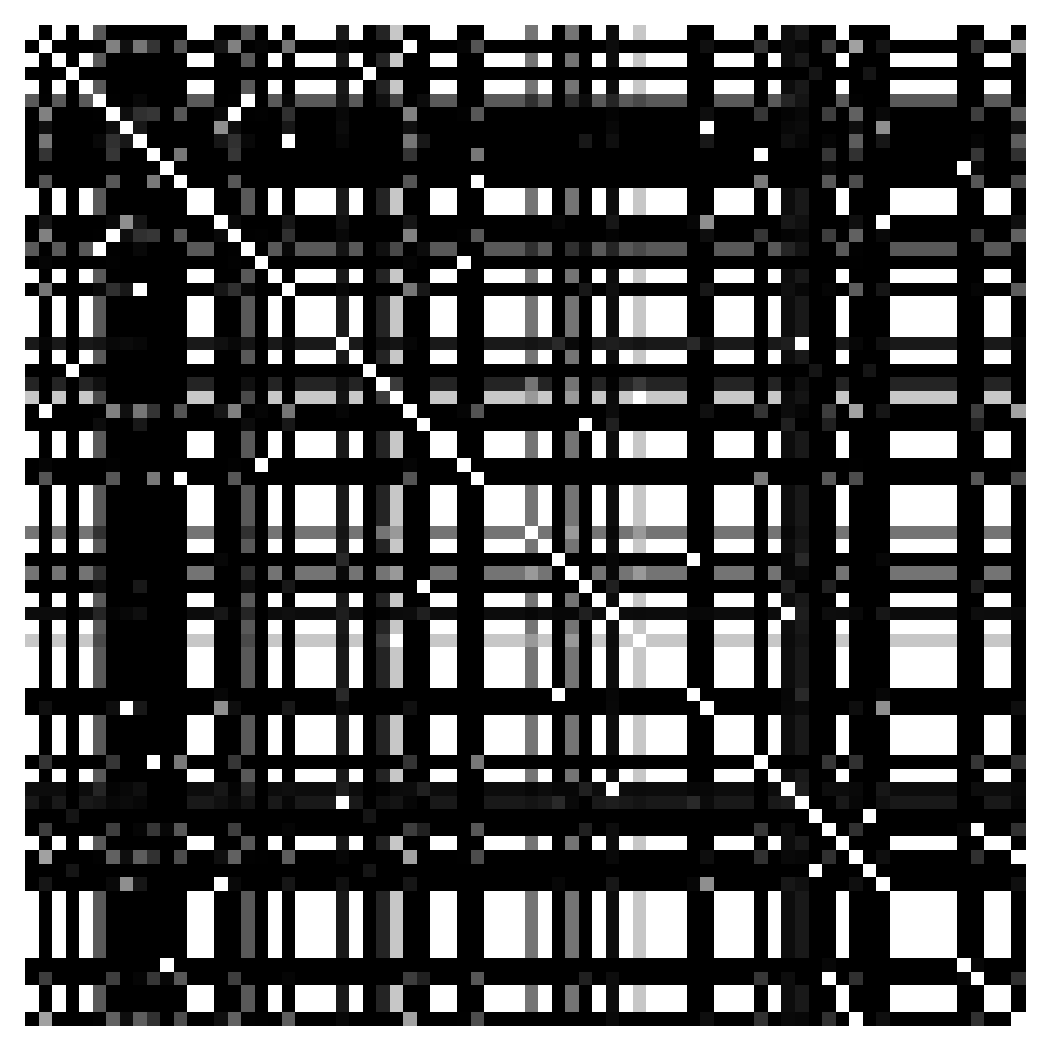
\includegraphics[width=\linewidth]{Figures/hadoop-runtime-commitX.pdf}
                \caption{Res. time}
        \end{subfigure}%
        \begin{subfigure}{0.19\textwidth}
                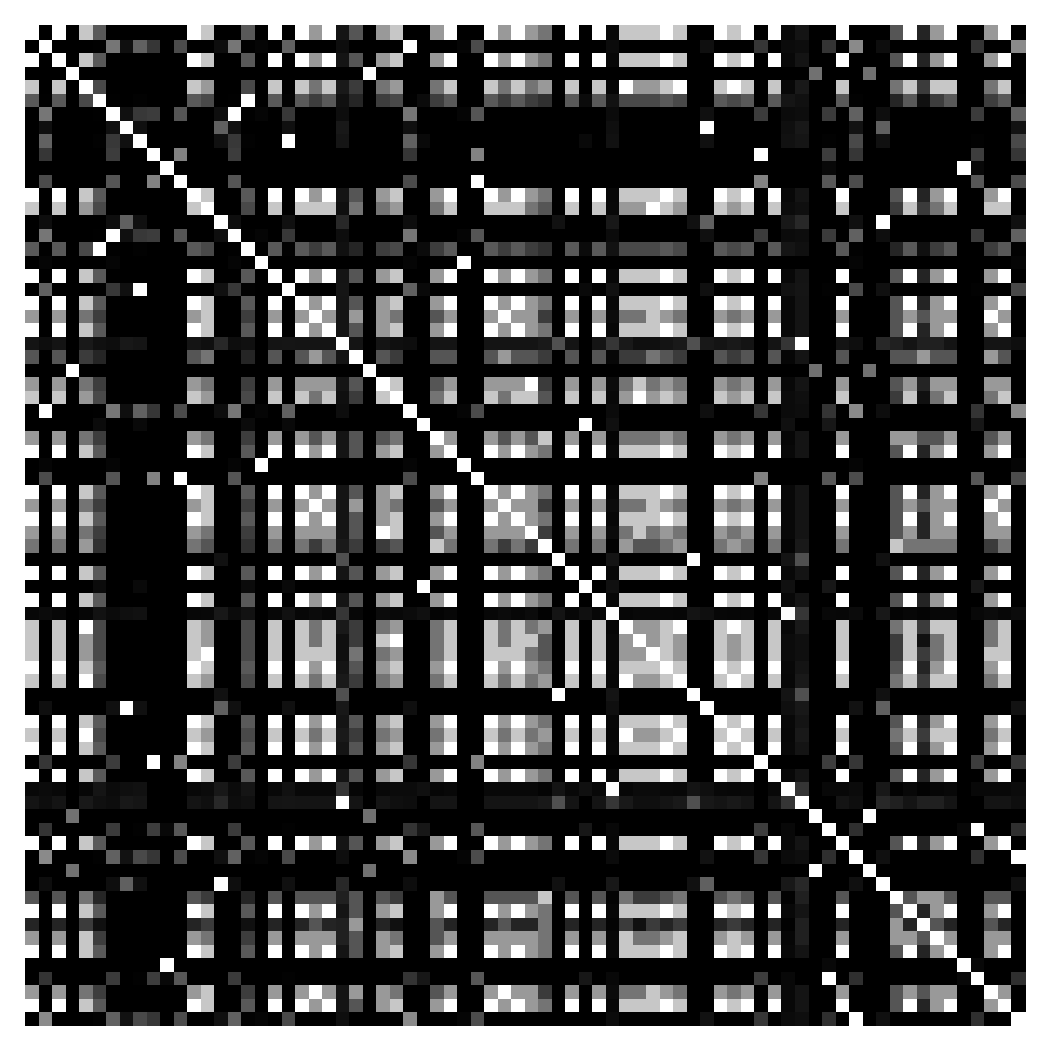
\includegraphics[width=\linewidth]{Figures/hadoop-cpu-commitX.pdf}
                \caption{CPU}
        \end{subfigure}%
        \begin{subfigure}{0.19\textwidth}
                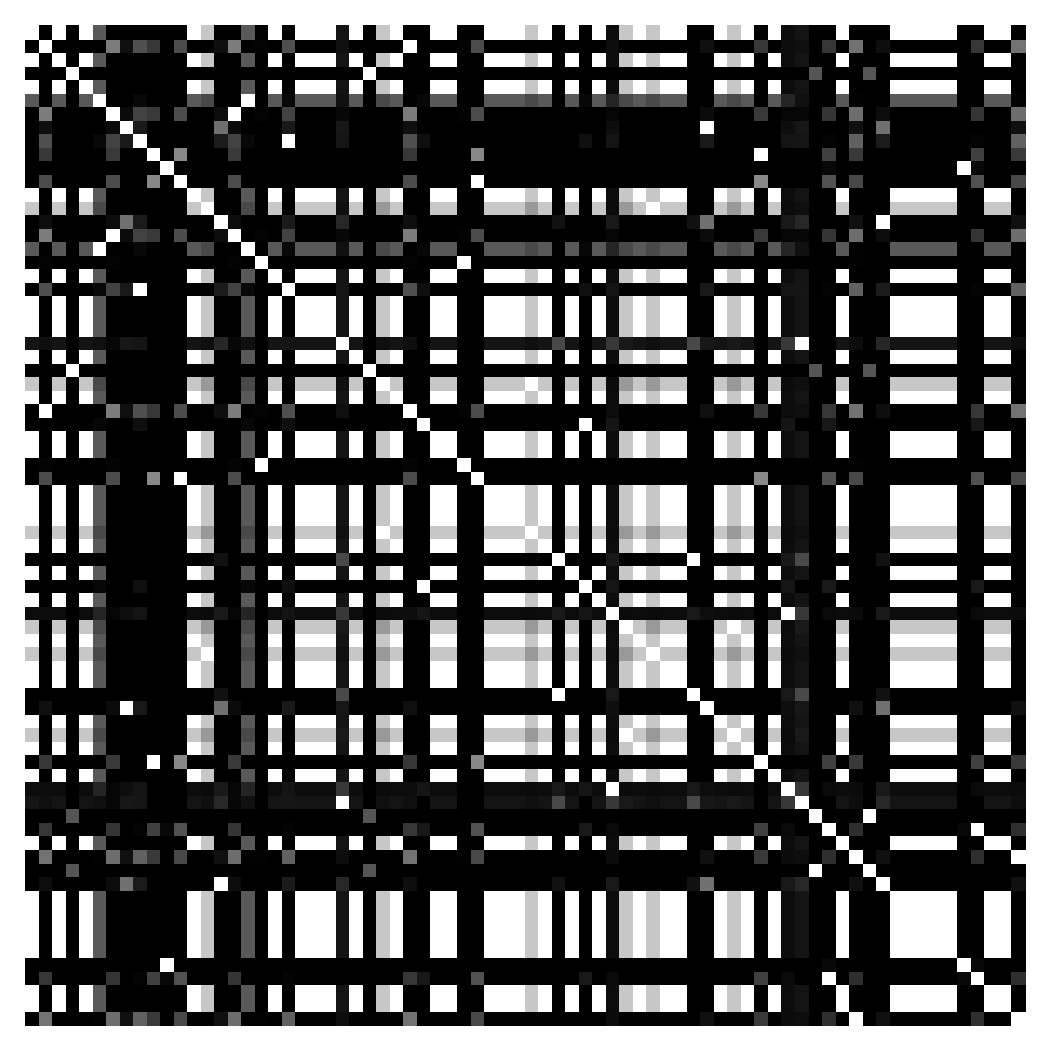
\includegraphics[width=\linewidth]{Figures/hadoop-mem-commitX.pdf}
                \caption{Memory}
        \end{subfigure}%
        \begin{subfigure}{0.19\textwidth}
                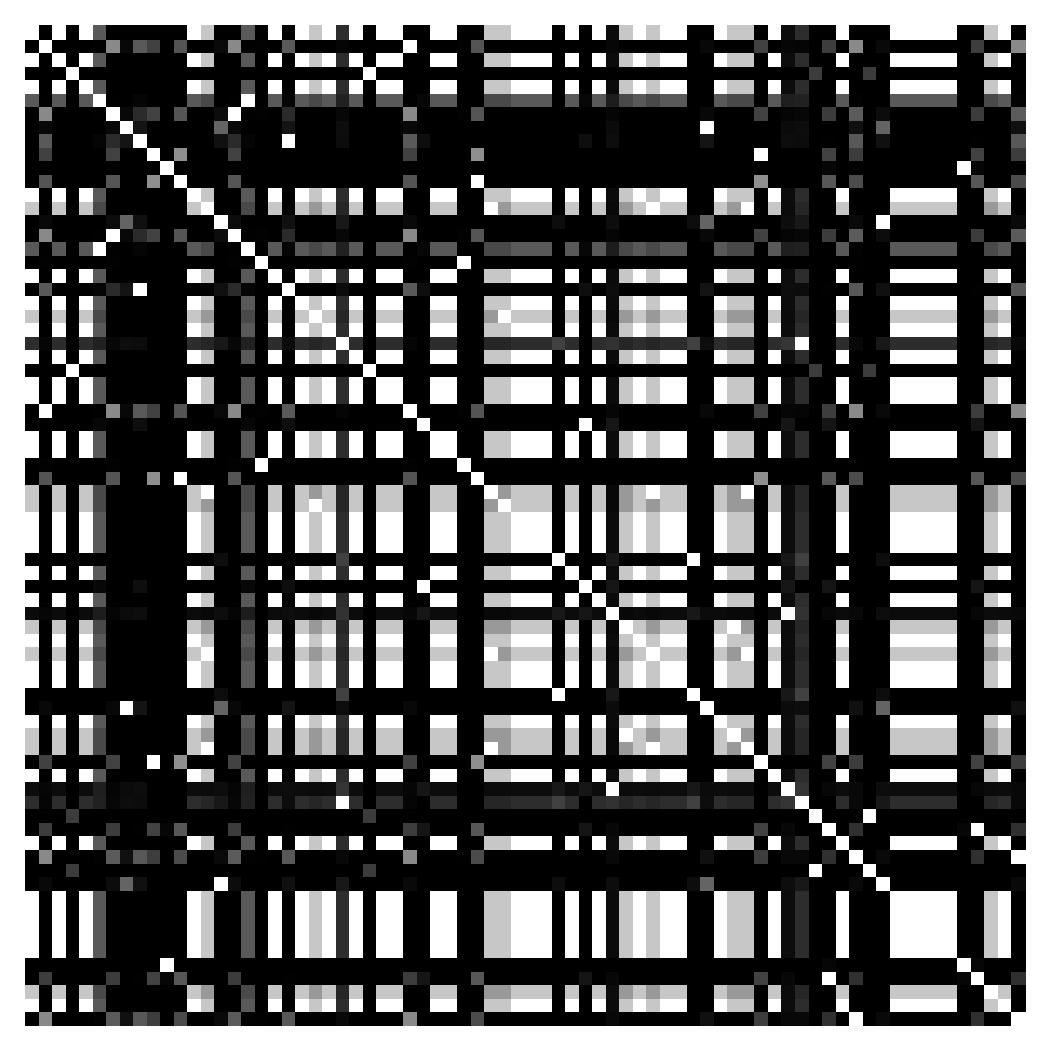
\includegraphics[width=\linewidth]{Figures/hadoop-ioread-commitX.pdf}
                \caption{I/O read}
        \end{subfigure}
        \begin{subfigure}{0.19\textwidth}
                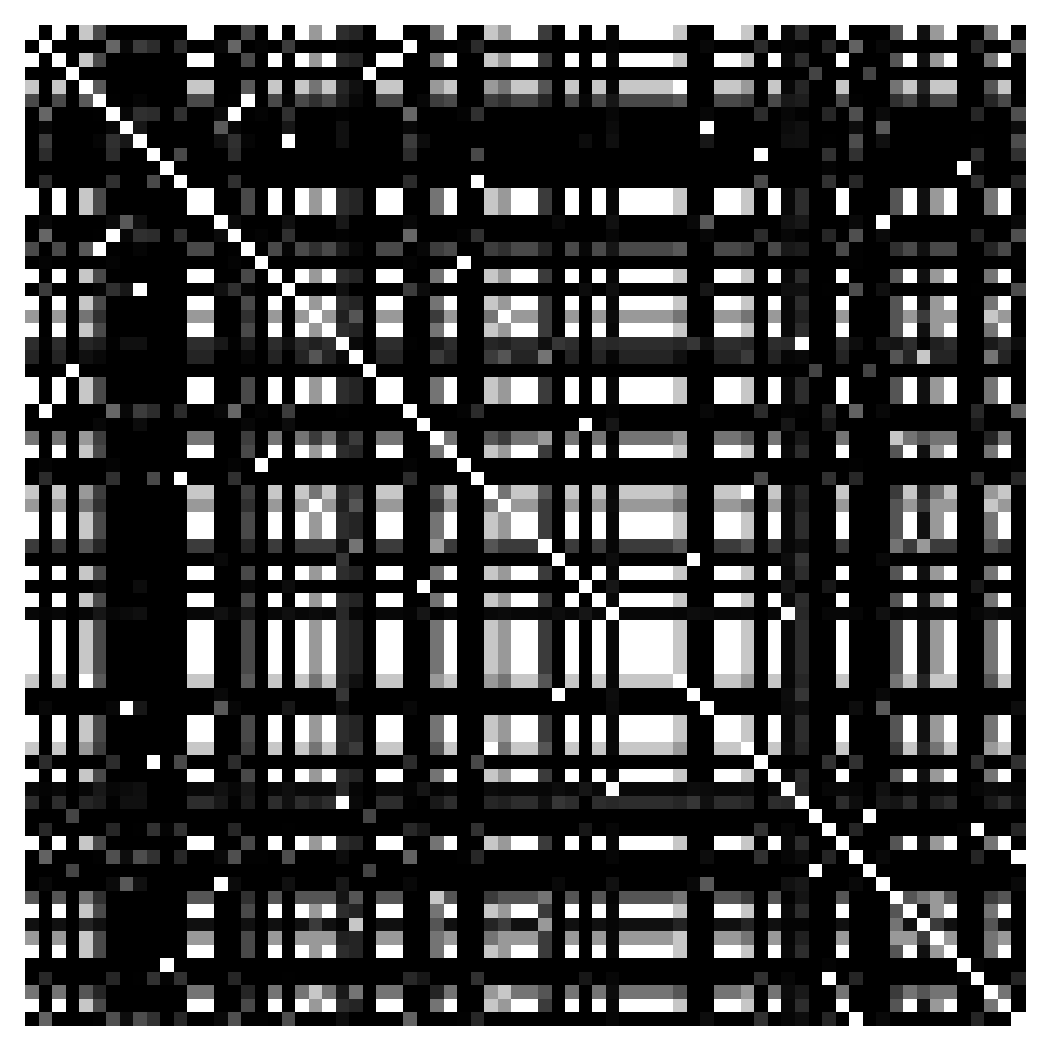
\includegraphics[width=\linewidth]{Figures/hadoop-iowrite-commitX.pdf}
                \caption{I/O write}
        \end{subfigure}
	\caption{Pairwise Jaccard distance between the $<$test, option, \inconsistent$>$ triplets of the studied commits of the \emph{Hadoop} system. The $x$-axis and $y$-axis show the studied commits, ordered chronologically from left to right on the $x$-axis and bottom to top on the $y$-axis. Each cell of the Figure refers to the Jaccard distance of any pair of commits: the darker the color is, the larger the distance is.}
	\label{fig:across-commit-hadoop}
% 	\vspace{-0.15cm}
\end{figure*}

\begin{figure*}[t]
	\centering
        \begin{subfigure}{0.19\textwidth}
                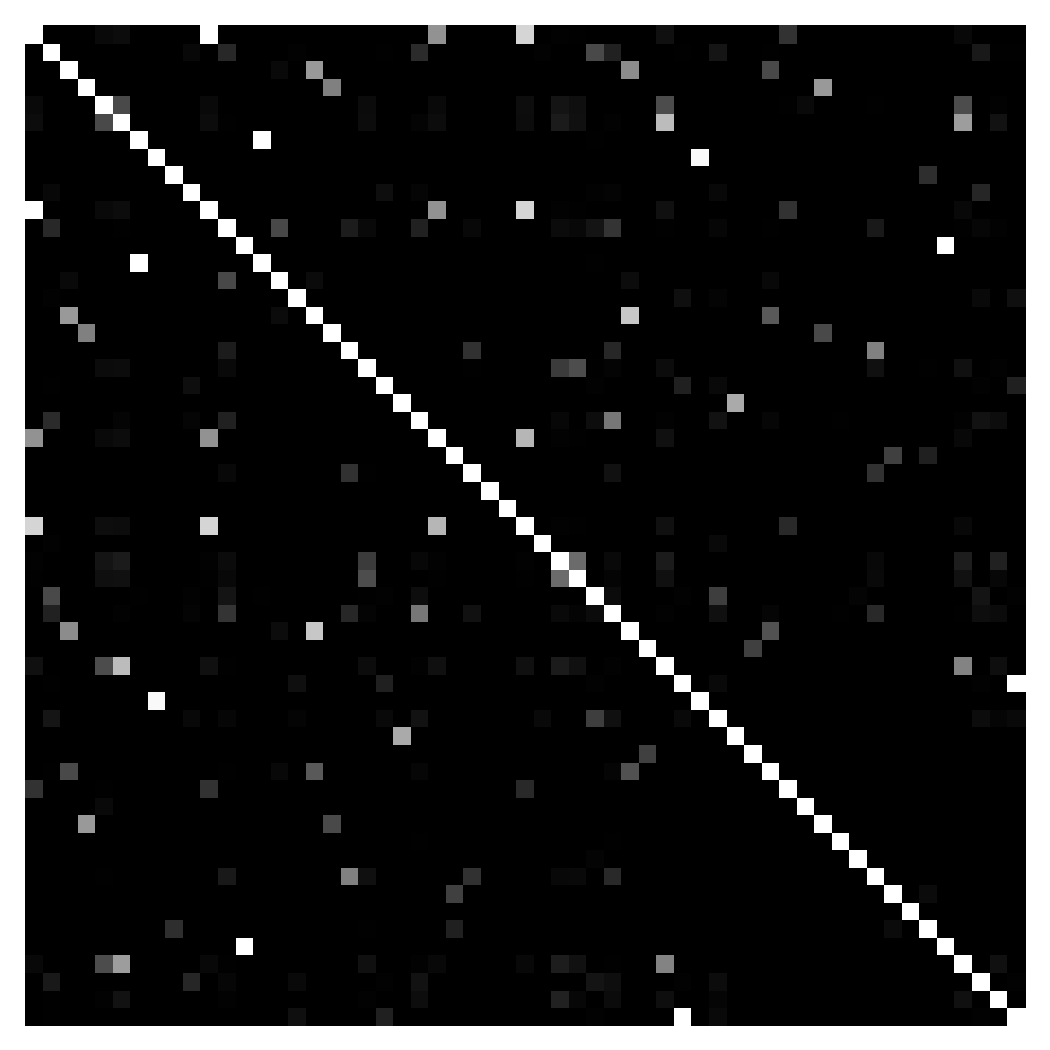
\includegraphics[width=\linewidth]{Figures/cassandra-runtime-commitX.pdf}
                \caption{Res. time}
        \end{subfigure}%
        \begin{subfigure}{0.19\textwidth}
                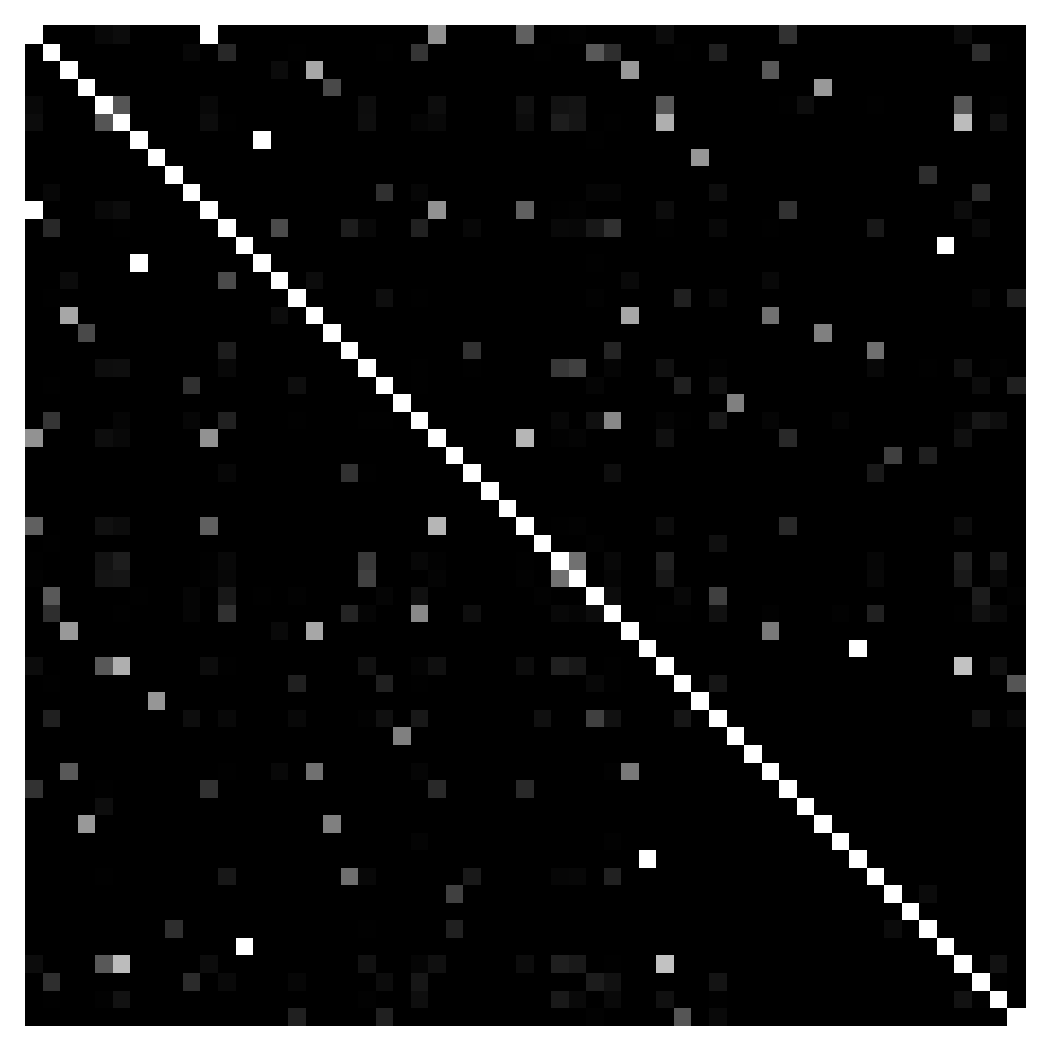
\includegraphics[width=\linewidth]{Figures/cassandra-cpu-commitX.pdf}
                \caption{CPU}
        \end{subfigure}%
        \begin{subfigure}{0.19\textwidth}
                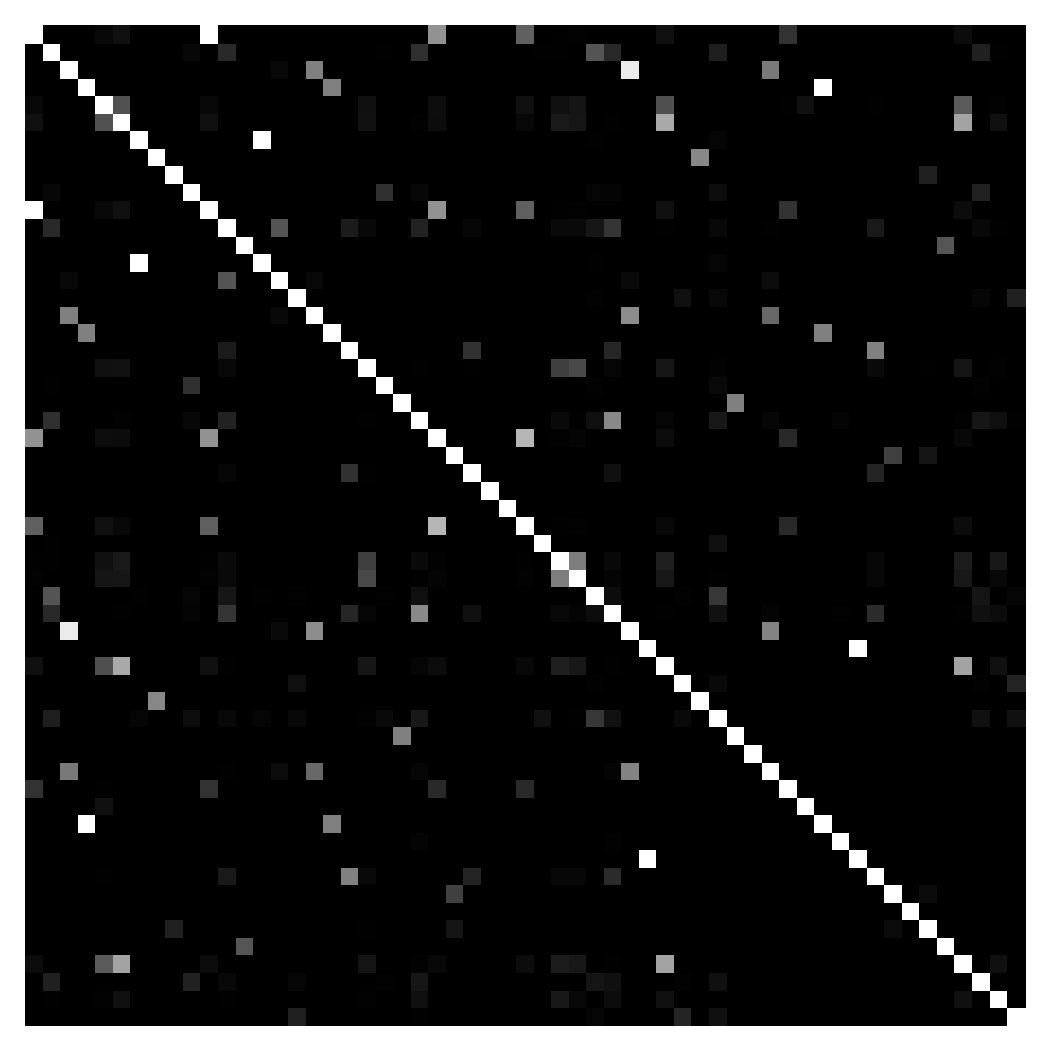
\includegraphics[width=\linewidth]{Figures/cassandra-mem-commitX.pdf}
                \caption{Memory}
        \end{subfigure}%
        \begin{subfigure}{0.19\textwidth}
                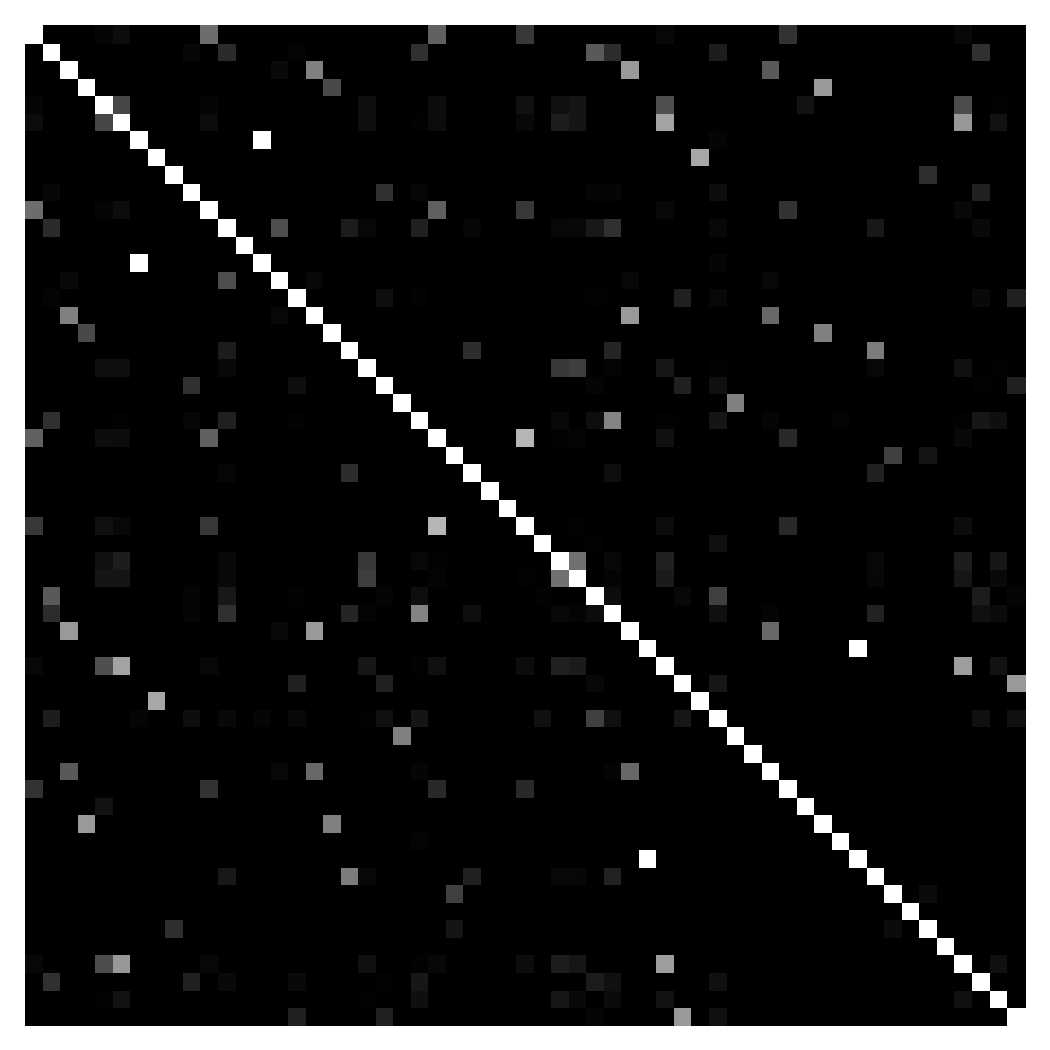
\includegraphics[width=\linewidth]{Figures/cassandra-ioread-commitX.pdf}
                \caption{I/O read}
        \end{subfigure}
        \begin{subfigure}{0.19\textwidth}
                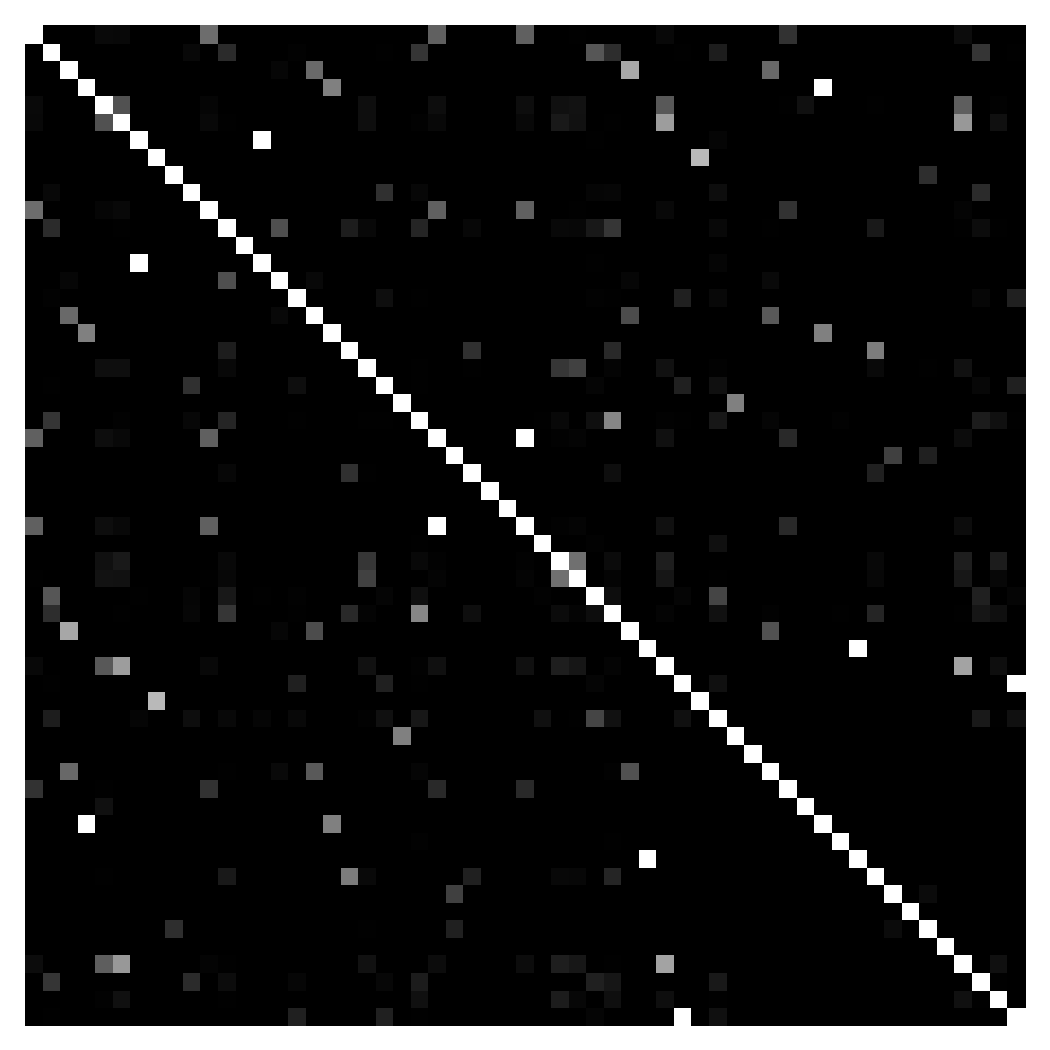
\includegraphics[width=\linewidth]{Figures/cassandra-iowrite-commitX.pdf}
                \caption{I/O write}
        \end{subfigure}
        
	\caption{Pairwise Jaccard distance between the $<$test, option, \inconsistent$>$ triplets of the studied commits of the \emph{Cassandra} system. The $x$-axis and $y$-axis show the studied commits, ordered chronologically from left to right on the $x$-axis and bottom to top on the $y$-axis. Each cell of the Figure refers to the Jaccard distance of any pair of commits: the darker the color is, the larger the distance is.}
	\label{fig:across-commit-cassandra}
\end{figure*}

%we can note from Figure~\ref{fig:across-commit-hadoop}
%and Figure~\ref{fig:across-commit-cassandra} that most of the pairs of commits (cells) have a small distance (light blue color), with only a limited number of cases (dark horizontal/vertical lines) that have substantially different regressing options. 


%\med{-----------}

%\noindent \textbf{Performance regression manifested under a subset of the possible configurations is common.} We observe that 69\% (51 out of 74) of the \emph{Hadoop} and 93\% (53 out of 57) of the \emph{Cassandra} commits have at least one configuration with a performance regression manifested by one of our five studied performance measurement and under one of the executed tests. Similarly, we observe that 69 out of 74 of the \emph{Hadoop} and 202 out of 216 of the \emph{Cassandra} unit tests show at least one performance regression through the whole history and across different configurations. Table~\ref{tab:dimemssion_regression} shows more details about how common the performance is manifested for the studied commits, tests, configurations, and options' values. 


%Almost all the options 100\% (122 out of 122) and 80\% (43 out of 54) of \emph{Hadoop} and \emph{Cassandra} options) lead at least once (in one commit and test) to a performance regression, which indicate how difficult it is to identify configurations that hide a performance regression. That is in particular since the number of possible values leading to such issues is just \med{xyz\%} and \med{xyz\%} for \emph{Hadoop} and \emph{Cassandra}, respectively. The number of options manifesting a performance regression in our studied dataset is large for all the performance metrics, when the optoins' values leading to a regression issue is small as shown in Table~\ref{tab:dimemssion_regression}. 


%\noindent \textbf{The set of configuration options that may cause the different manifestations of performance regressions are not similar between commits.}
%The results of the number of commits, tests, and options with performance regressions are shown in Table~\ref{tab:dimemssion_regression}. \bram{where do these numbers occur in the table?} We note that 51 out of 74 (69\%) of the commits from \emph{Hadoop} and 53 out of 57 (93\%) of the commits from \emph{Cassandra} have at least one option with performance regression in any of the performance metrics. \bram{other observations in the table (a lot of numbers)?}

%When we measure the configuration options with performance regressions across commits of the subject systems, we find that the configuration options with performance regressions are not consistent across consecutive commits (see Figure~\ref{fig:across-commit-hadoop} and Figure~\ref{fig:across-commit-cassandra}). 
%\med{move to the figure caption}



%\med{I stopped here for this RQ, I would suggest to consider the value of options as well for figure 2. that can give better results. According to the previous paragraph, a lot of options have a regression somewhere but few values have a regression.}For instance, the configuration options with performance regressions are not consistent across consecutive commits, as shown in Figure~\ref{fig:across-commit-hadoop} and Figure~\ref{fig:across-commit-cassandra}. 


%\med{to review after discussing/addressing my previous comment}The two figures show that the set of configuration options that cause performance regressions mostly are the same in between commits. In particular, we can note from Figure~\ref{fig:across-commit-hadoop}
%and Figure~\ref{fig:across-commit-cassandra} that most of the pairs of commits (cells) have a small distance (light blue color), with only a limited number of cases (dark horizontal/vertical lines) that have substantially different regressing options. For example, in the case of response time for Hadoop, we notice two commits with entirely different sets of regressing options from the others, while the other options' regressing have substantial overlap. Response time for Cassandra has a higher number of medium to dark colored cells, but overall still features a majority of ligthly colored cells. In contrast, the plot for I/O write for Hadoop features a high density of dark lines, suggesting less consistent regressions.

%\med{That should move to the motivation of RQ2}These observations suggest that prediction models might obtain good performance in pinpointing regressing options for the cases with few dark lines. Especially Hadoop features substantial overlap between commits in terms of regression options. The next RQ builds and empirically validates such prediction models, aimed at warning developers of potential performance regressions for specific configuration options.%However, there exist a set of pairs of commits that have a large distance (dark blue color cell). For example, we find that \jinfu{give an example.}
 
%\noindent\med{I don't see the value for this manual analysis. What already exists (too much options, few values, and a lot of differences among the commits especially for Hadoop and Cassand I/O write) is good enough to motivate an automatic approach to predict the regressions.} \textbf{place holder for the manual examination} \bram{manually analyze interesting cases of response time Hadoop vs. Cassandra? i.e., few options responsible for large changes?} 

%To further understand the reason that configuration options cause different manifestations of performance regression between commit pairs, 
In order to understand why different commits show inconsistent $<$test, option, \inconsistent$>$ triplets, 
we manually analyze some commits that show the largest Jaccard distance from other commits (i.e., with dark horizontal/vertical lines in Figure~\ref{fig:across-commit-hadoop} and Figure~\ref{fig:across-commit-cassandra}). We focused on the response time measure in our manual analysis because response time is a typical performance metric that may directly affect user experience. %\bram{because \dots}. 
In particular, there are two and six commits with large Jaccard distance ($>0.8$) to all other commits in \emph{Hadoop} and \emph{Cassandra}, respectively. 
%We find that many of the configuration options manifest performance regression in those commits. 
For \emph{Hadoop}, we find that most of the options cause \inconsistent in the test named \emph{TestKMS.java} in the \emph{Hadoop-common} sub-project. 
%Therefore, configuration practitioners can assign more focuses on the test \emph{TestKMS.java}. 
Then, we pick up one\footnote{\url{https://github.com/apache/hadoop/commit/b17d365f}} out of the two commits of \emph{Hadoop} to manually examine the impacted tests, configuration option and the commit changes based on our constructed mappings in Section~\ref{sec:impactedtests}. %\bram{what was studied for the other cases?}. %\heng{Check if the following is right}
We find that the studied options that cause \inconsistent are related to connection time, such as the options \emph{dfs.ha.fencing.ssh.connect-timeout} and \emph{fs.s3a.connection.timeout}. By examining the code in the test \emph{TestKMS.java}, we find that \emph{TestKMS.java} loads the connection timeout configuration options. And the code changes in this commit trigger the test case in the test \emph{TestKMS.java}. 
Thus, the commits that impact such connection time-related options and the test may lead to \inconsistent problems while other commits may not lead to the same \inconsistent. %\bram{why would that be? rare type of change + particularly performance-impacting test?}

For \emph{Cassandra}, we select one commit\footnote{\url{https://github.com/apache/cassandra/commit/0fe82be8}} with the largest Jaccard distance to other commits. Our results show that two tests named \emph{EmbeddedCassandraServiceTest} and \emph{DebuggableScheduledThreadPoolExecutorTest} manifest the largest performance regression regarding options \emph{max\_hints\_file\_size\_in\_mb} and \emph{memtable\_heap\_space\_in\_mb}, respectively. By manually examining the commit changes covered by the tests, we find that there exist code changes in the method \emph{start} within the Java file \emph{EmbeddedCassandraService.java}\footnote{\url{https://github.com/apache/cassandra/blob/0fe82be83cceceb12172d63913388678253413bc/src/java/org/apache/cassandra/service/EmbeddedCassandraService.java\#L53}}. %Such a change adds function calls to initialize the options and leads to performance regressions. 
Such code changes trigger the test cases to load and initialize options in the impacted tests \emph{EmbeddedCassandraServiceTest} and \emph{DebuggableScheduledThreadPoolExecutorTest}, which lead to performance regression. %\bram{same question as before, why do we see this for this file/test?}
In particular, 69\% of commits in \emph{Hadoop and }96\% of commits in \emph{Cassandra} have a Jaccard distance more than 0.5. Such results imply that different commits may lead to different options and tests that exhibit \inconsistent problems. %\bram{rather general/trivial finding, can we be more specific?}






\begin{comment}
\begin{table}[t]
  \centering
  \caption{Number of executed tests with performance regression \bram{following is confusing:} in different configuration options with different values}
  \tabcolsep=0.1cm
  \begin{tabular}{|c|c|c|r|c|r|c|r|c|r|c|r|}
    \hline
    \multirow{2}{*}{subject} & \multirow{2}{*}{\begin{tabular}[c]{@{}c@{}} \#Executed\\ tests\end{tabular}} & \multicolumn{2}{c|}{Response time}   & \multicolumn{2}{c|}{CPU}   & \multicolumn{2}{c|}{Memory}& \multicolumn{2}{c|}{I/O   read} & \multicolumn{2}{c|}{I/O   write}\\ \cline{3-12} 
     && large  & \multicolumn{1}{c|}{medium} & large  & \multicolumn{1}{c|}{medium} & large  & \multicolumn{1}{c|}{medium} & large  & \multicolumn{1}{c|}{medium} & large  & \multicolumn{1}{c|}{medium} \\ \hline
    Hadoop& \multicolumn{1}{r|}{13566}  & \multicolumn{1}{r|}{1708} & 128 & \multicolumn{1}{l|}{4180} & 342 & \multicolumn{1}{r|}{836}  & 562 & \multicolumn{1}{r|}{966}  & 178 & \multicolumn{1}{r|}{2626} & 292 \\ \hline
    Cassandra & \multicolumn{1}{r|}{30825}  & \multicolumn{1}{r|}{2353} & \multicolumn{1}{r|}{1852}   & \multicolumn{1}{r|}{6116} & \multicolumn{1}{r|}{2049}   & \multicolumn{1}{r|}{2729} & \multicolumn{1}{r|}{1749}   & \multicolumn{1}{r|}{5573} & \multicolumn{1}{r|}{2176}   & \multicolumn{1}{r|}{5595} & \multicolumn{1}{r|}{1829}   \\ \hline
    \end{tabular}
  \label{tab:perf_regression}
\end{table}
\end{comment}


% \begin{figure*}[tbh]
% 	\centering
% 		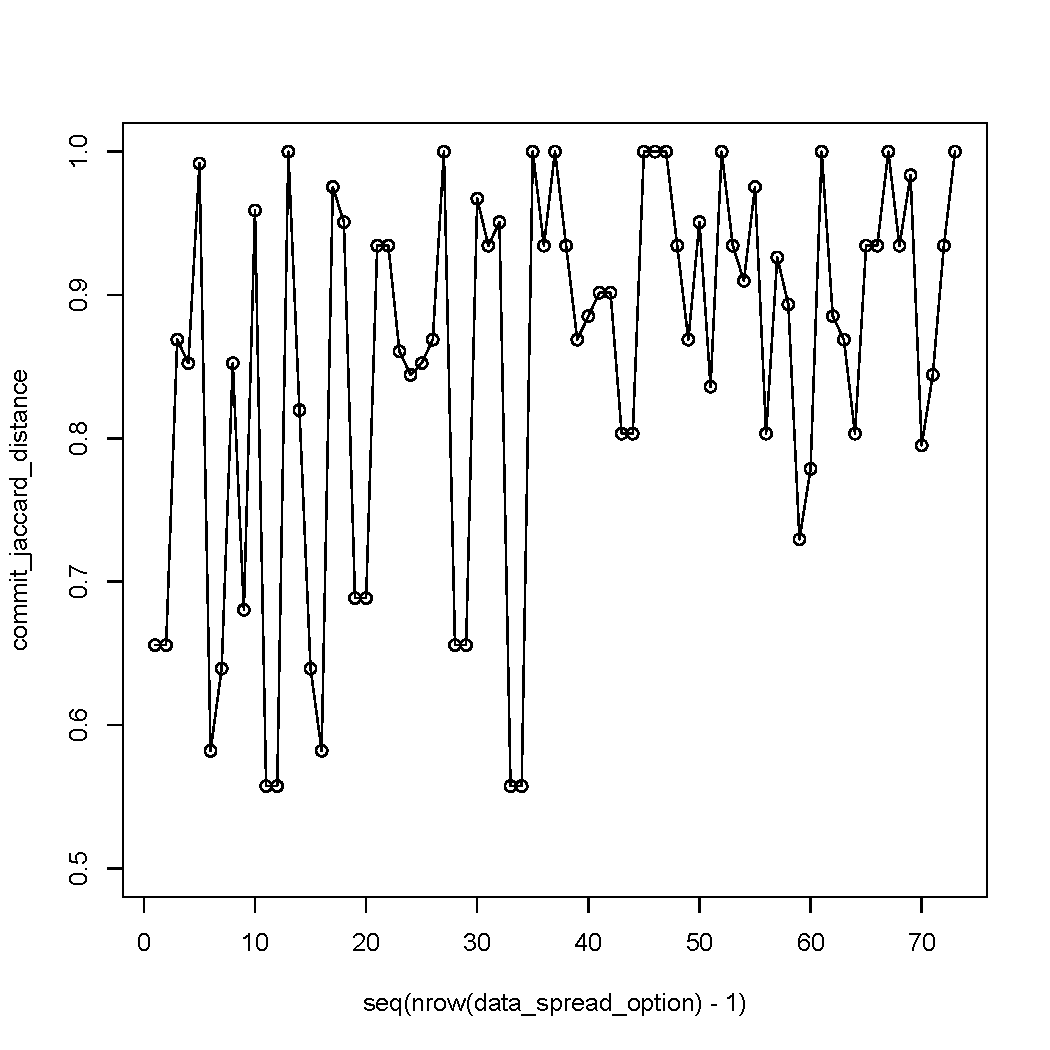
\includegraphics[width=.9\textwidth]{Figures/hadoop_restime.pdf}
% 	\caption{option change across commits.} 
% 	\label{fig:across-commit} 
% \end{figure*}



\begin{Summary}{Summary of Preliminary Study}{}
\inconsistent is a common problem and it is difficult to manually identify \inconsistent without exhaustively running the tests. Our results suggest the need for an approach that automatically identifies which \instance manifests an \inconsistent. 
\end{Summary}


%%% Local Variables:
%%% mode: latex
%%% TeX-master: "../main"
%%% End:
